\documentclass[12pt,letterpaper]{article}

% --- Packages ---
\usepackage[utf8]{inputenc}
\usepackage[top=1in, bottom=1in, left=1.25in, right=1.25in]{geometry}
\usepackage{amssymb,amsmath,amsthm}
\usepackage{graphicx}
\usepackage{float}
\usepackage{xcolor}
\usepackage{titlesec}
\usepackage{setspace}
\usepackage{hyperref}
\usepackage{cite} % For basic numerical citations
% Use the same font style as your homework
\usepackage{times,txfonts}

% --- Formatting ---
\onehalfspacing % Standard for literature reviews
\hypersetup{
    colorlinks=true,
    linkcolor=blue,
    filecolor=magenta,      
    urlcolor=cyan,
    citecolor=blue,
}

% --- Custom Header (Matches your HW style) ---
\usepackage{fancyhdr}
\pagestyle{fancy}
\fancyhf{}
\fancyhead[L]{Turbulent Flows: Literature Review}
\fancyhead[C]{March 2026}
\fancyhead[R]{Stefano Fochesatto}
\fancyfoot[C]{\thepage}
\headheight 15pt

% --- Math Shortcuts (From your template) ---
\newcommand{\Reals}{\ensuremath{\mathbb R}}
\let\RR\Reals

% --- Title Info ---
\title{\Large \textbf{A hybrid RANS-LES approach with delayed-DES and wall-modelled LES capabilities}}
\author{Stefano Fochesatto \\ \small University of Colorado Boulder}
\date{\today}

\begin{document}

\maketitle



\section{Introduction} 
A hybrid RANS-LES approach with delayed-DES and wall-modelled LES capabilities by Shur et al.~\cite{shur2008hybrid} presents a new computational fluid dynamics modelling strategy called Improved Delayed Detached-Eddy Simulation (IDDES). This method provides a unified framework for hybrid RANS-LES models. Before this paper, there were two primary types of hybrid models aimed at mitigating the power-dependent Reynolds number cost of wall-resolved LES: Delayed Detached-Eddy Simulation (DDES) and Wall-Modelled Large Eddy Simulation (WMLES). Both methods essentially stitch together a RANS model near the wall with an LES model in the outer domain. However, they fundamentally differ in their target applications and how this transition is prescribed.

DDES is primarily designed for high-Reynolds-number massively separated flows. In this approach, the entire attached boundary layer is handled by the RANS model, and the simulation only switches to LES in separated flow regions. The transition is seamless and determined primarily by the local grid spacing relative to the modeled turbulent length scales. Conversely, traditional WMLES approaches aim to resolve most of the boundary layer with LES, using RANS only in a much thinner near-wall region. Prior to IDDES, many WMLES methods were zonal, requiring practitioners to explicitly prescribe the RANS and LES interface \emph{a priori}, or they relied on highly specific, "channel-friendly" steps that struggled with complex geometries. Furthermore, when seamless models like DES were applied as wall models, they suffered  from an issue called the "log-layer mismatch" (LLM), which is essentially a discontinuity between the RANS-modeled inner log-layer and the LES-resolved outer log-layer that resulted in an under-prediction of skin friction by up to 15-20\% \cite{shur2008hybrid}.

To resolve these limitations, Shur et al. introduce IDDES, a non-zonal model that mathematically unifies DDES and WMLES. The key contribution of this paper is the definition of the subgrid length-scale, $\Delta$. Previous seamless models relied solely on maximum grid cell dimensions, the IDDES subgrid length-scale explicitly incorporates the distance to the wall, $d_w$. This new length scale along with some choices of dynamic empirical blending functions, the model automatically detects whether the inflow contains turbulent content. It then seamlessly transitions between a DDES mode for attached flows without turbulent content and a WMLES mode for resolving active boundary-layer turbulence.

Before detailing the specific contributions made in Shur et al. we must first understand the foundational RANS and LES techniques that IDDES builds upon.






\section{Basic Techniques}
\subsection{\textbf{RANS: Reynolds-Averaged Navier-Stokes}} The main idea behind RANS is to simplify the Navier-Stokes equations by considering the velocity $U_i$ and decomposing it into a time-averaged mean component $\langle U_i\rangle$ and its corresponding fluctuation $u_i$, i.e.
\begin{equation}
    U_i = \langle U_i \rangle + u_i.  
\end{equation}
This form for describing the velocity field is called the \emph{Reynolds decomposition}. Deriving the governing Reynolds equations for the RANS technique involves simply substituting this form into Navier-Stokes equations and taking a mean as is done in Chapter 4 of \cite{pope2000}. The following equations are derived as a result: \\
From the mean continuity equation,
\begin{equation}
    \nabla \cdot \langle \bf{U} \rangle = 0.
\end{equation}
From the mean momentum equations, 
\begin{equation}
    \frac{\bar{D}\langle U_j\rangle}{\bar{D}t} = \nu \nabla^2\langle U_j\rangle - \frac{\partial \langle u_iu_j\rangle}{\partial x_i} - \frac{1}{\rho} \frac{\partial \langle p\rangle }{\partial x_j}
\end{equation}
These four equations result in more than four unknowns because of the additional terms from the \emph{Reynolds stresses} terms $\langle u_i u_j \rangle$. This issue is often referred to as \emph{the closure problem}, in which there are several models for how these unknowns can be determined or approximated under different modeling hypothesis and constraints. Shur et al.~\cite{shur2008hybrid} mentions two RANS models, the SA (Spalart-Allmaras) Model and the MSST (Menter's Shear Stress Transport) $k - \omega$ Model. Both are described in moderate detail within Section 10.5 of Pope \cite{pope2000} however we will recall them in brief below. \\
\subsubsection{\textbf{$k-\omega$ Model}} In addition to the averaged mean momentum and mean continuity equations described above two model stransport equations, the first for turbulent kinetic energy $k$
\begin{equation}
     \frac{\bar{D}k}{\bar{D}t} = \nabla \cdot \left(\frac{\nu_T}{\sigma_k}\right) + \mathcal{P} - \omega
\end{equation}
where turbulent viscosity is defined by $\nu_T = ck^{1/2}\ell_m$ and of course $\ell_m(\bf{x}, t)$ is a specified mixing length.
\begin{equation}
    \frac{\bar{D}\omega}{\bar{D}t} = \nabla \cdot \left(\frac{\nu_T}{\sigma_\omega} \nabla \omega \right) + C_{\omega 1}\frac{\mathcal{P}\omega}{k} - C_{\omega 2} \omega^2. 
\end{equation}
While technically this is the Wilcox $k - \omega$ \cite{Wilcox93} the Menter model uses a blending function applied to the $C_{\omega2} \omega^2$ term to transition between the $k-\omega$ model near the wall to the $k-\epsilon$ model away from the wall. All this to say the general scheme for a two-equation turbulent viscosity involves, solving the model transport equations for $\omega$ then $k$, defining turbulent viscosity via $\nu_T = ck^{1/2}\ell_m$, obtaining the Reynolds stress terms via the turbulent-viscosity hypothesis, 
\begin{equation}
    \langle u_i u_j \rangle = \frac{2}{3} k \delta_{ij} - \nu_T \left(\frac{\partial \langle U_i \rangle }{\partial x_j} + \frac{\partial \langle U_j \rangle}{\partial x_i} \right).
\end{equation}
and finally solving the original 4 equations for $\langle   \bf{U}\rangle$ and $\langle p \rangle$. \\

\subsubsection{\textbf{SA (Spalart-Allmaras) Model}} The SA model \cite{SAModel} is a one-equation model for $\nu_T$ given by, 
\begin{equation}
    \frac{\bar{D}\nu_T}{\bar{D}t} = \nabla \cdot \left(\frac{\nu_T}{\sigma_\nu} \nabla \nu_T \right) + S_\nu
\end{equation}
Where the source term $S_\nu$ depends on the laminar and turbulent viscosities $\nu$ and $\nu_T$; the mean vorticity $\Omega$; the turbulent viscosity gradient $|\nabla \nu_T|$; and the distance to the nearest wall, $\ell_w$. 


\subsection{\textbf{LES: Large-Eddy Simulation}}Recall that while Direct Numerical Simulation (DNS) is highly accurate because it resolves all scales of motion without modeling, its computational cost is prohibitive for high-Reynolds-number engineering applications. As Piomelli and Balaras \cite{piomelli2002wall} note, the number of grid points required in three dimensions scales proportionally to $Re_L^{9/4}$ (where $Re_L$ is the Reynolds number based on the integral scale). When factoring in the temporal resolution required to capture these dynamics, the total computational cost increases approximately as the cube of the Reynolds number \cite{pope2000}. Consequently, DNS is practically restricted to flows with $Re_L = \mathcal{O}(10^4)$ \cite{piomelli2002wall}. Furthermore, nearly all of this computational effort is expended resolving the smallest, dissipative motions \cite{pope2000}, whereas the energy and anisotropy of the flow are predominantly contained in the larger scales. Large-Eddy Simulation (LES) provides an intermediate technique between DNS and the Reynolds-Averaged Navier-Stokes (RANS) equations. In the LES method, we aim to explicitly compute the large, energy-carrying motions by applying spatial filtering to the Navier-Stokes equations, while the effects of the smaller-scale residual motions are represented with a simpler model. This approach is highly effective because the smaller subgrid scales tend to be more isotropic and homogeneous, making them much more amenable to universal modeling than the large, geometry-dependent scales \cite{piomelli2002wall}. The four conceptual steps of LES modeling, as outlined in Chapter 13 of \cite{pope2000}, go as follows:
\begin{enumerate}
    \item We define a filtering operation to decompose the velocity $\mathbf{U}$ into the sum of a filtered component $\bar{\mathbf{U}}$ and a residual component $\mathbf{u'}$. 
    \item The momentum and continuity equations in terms of the filtered velocity are derived via substitution of the filtered decomposition. The momentum equation will contain the \emph{residual-stress tensor} (or subgrid-scale (SGS) stress tensor). 
    \item We close the equations by modelling the residual stress with another simpler model.
    \item The modelled filtered equations are then solved numerically. 
\end{enumerate} 

Chapter 13 of Pope \cite{pope2000} elaborates further on LES methods, however I will define briefly a few key equations and relate them to the four conceptual steps introduced above. The general filtering operation as discussed in Section 13.2.1 of Pope is defined as a convolution of the velocity field $\mathbf{U}$ and some specified filter function $G$ which specifies a filter width $\Delta$ and has a normalization condition:

\begin{equation}
    \bar{\mathbf{U}} = \int G(\mathbf{r}, \mathbf{x})\mathbf{U}(\mathbf{x - r}, t) d\mathbf{r}, \quad\quad \int G(\mathbf{r}, \mathbf{x}) d\mathbf{r} = 1
\end{equation}

Here $\bar{\mathbf{U}}$ is the filtered velocity, and we take $\mathbf{u'}$ to be the associated residual, leaving us with a decomposition that is analogous to the Reynolds Decomposition. Similarly, via substitution into the Navier-Stokes equations we obtain filtered conservation equations.\\

The filtered continuity equation,
\begin{equation}
    \frac{\partial \bar{U}_i}{\partial x_i} = 0. 
\end{equation}

The filtered momentum equations,
\begin{equation}
    \frac{\bar{D}\bar{U}_j}{\bar{D}t} = \nu \frac{\partial^2 \bar{U}_j}{\partial x_i \partial x_i} - \frac{\partial \tau^r_{ij}}{\partial x_i} - \frac{1}{\rho} \frac{\partial \bar{p}}{\partial x_j}. 
\end{equation}

where the substantial derivative based on filtered velocity is,
\begin{equation}
    \frac{\bar{D}}{\bar{D}t} \cong \frac{\partial}{\partial t} + \bar{\mathbf{U}}\cdot \nabla. 
\end{equation}

The term $\tau^r_{ij}$ is referred to as the residual-stress tensor and is again, like the RANS equations, subject to a closure problem which we must use a simpler model to solve. 

\subsubsection{The Smagorinsky Model} 
As described in Chapter 13.4 of \cite{pope2000}, the Smagorinsky model can be viewed in two parts. First, the linear eddy-viscosity model,
\begin{equation}
    \tau^r_{ij} = -2\nu_r\bar{S}_{ij}. 
\end{equation}
This relates the residual stress tensor with the filtered strain rate tensor. Analogously applying a mixing length hypothesis we can model the eddy-viscosity of the residual motions $\nu_r$, 

\begin{align}
    \nu_r &= \ell_s^2\bar{\mathcal{S}},\\
    &=(C_s\Delta)^2\bar{\mathcal{S}}.
\end{align}

Where $\bar{\mathcal{S}} = (2\bar{S}_{ij}\bar{S}_{ij})^{1/2}$ is the characteristic filtered strain rate tensor, $\ell_s$ is the \emph{Smagorinsky lengthscale} which is analogous to the mixing length and is proportional to the filter width $\Delta$, and $C_s$ is the dimensionless \emph{Smagorinsky constant}.

\section{Hybrid Models: Detached Eddy Simulations}

Spalart et al. \cite{} proposed a hybrid RANS/LES method referred to as Detached Eddy Simulation (DES). Essentially for wall bounded flows a Wall-Resolved LES (WRLES) requires a grid resolution that approaches DNS-like density in the inner boundary layer. As estimated by Choi and Moin \cite{choi2012grid}, the number of grid points required to resolved an attached boundary layer scales approximately as $Re^{13/7}$. For typical engineering applications this requirement renders WRLES computationally infeasible. As an alternative DES invkes a RANS closure near solid surfaces where the flow is attached, and a SGS closure (LES type model) in the detached flow regions. 

\begin{figure}[H]
    \begin{center}
        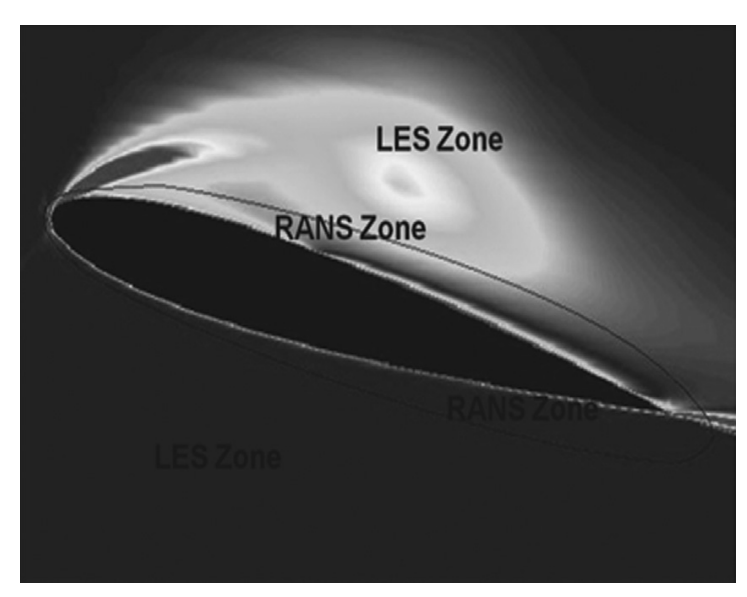
\includegraphics[width = .5\textwidth]{DES.png}
        \caption{DES Concepts \cite{SciDirectOverview}}
    \end{center}
\end{figure}

To accomplish this transition Spalart et al. proposes modifying the turbulence length scale $\ell_W$ of the SA model with the following,
\begin{equation}
    \ell_{\text{DES}} = \min\left\{\ell_W, \Delta_{\text{DES}}\right\}, \quad \Delta_{\text{DES}} = C_{\text{DES}}\Delta_{\max}, \quad \Delta_{\max} = \max\left\{\Delta_x, \Delta_y, \Delta_z\right\}
\end{equation}
Where $C_{DES}$ is an empirical constant and $\Psi$ is a low Reynolds number correction term. The details of a RANS model are discussed in Spalart et al. however the main takeaway is that DES models are derived by modifying the length scales of RANS models, and doing so creates a region detached from the wall, where the model behaves like an LES model. 

One of the problems that the original DES approach has, and is addressed with Delayed Detached Eddy Simulation (DDES) (spalart 06) is when the grid is locally refined, to say resolve some region of high geometric curvature, the maximum grid length cell is minimized and the switch between the RANS and LES behavior happens within the attached boundary layer. Grids that encounter this issue are often refered to as \emph{ambiguous grids}. To address this issue proposes the following length scale, 
\begin{equation}
    \ell_{\text{DDES}} = \ell_{W} - f_d \max\left[0, \ell_{W} - \Delta_{\text{DES}} \right]
\end{equation}
    Where the shielding function, $f_d$ is defined as, 
    \begin{equation}
f_d = 1 - \tanh\left[ (C_{f_d} r_d)^3 \right], \qquad r_d = \frac{\mu + \mu_t}{\bar{\rho} (\kappa d)^2 \max \left[ \sqrt{\frac{\partial u_i}{\partial x_j} \frac{\partial u_i}{\partial x_j}} , 10^{-10} \right]}
    \end{equation}
    Here $C_{f_d} = 8$ and the argument $r_d$ is close to unity in the sub-lyer and logarithmic portions of the boundary layer, and asymptotes to zero as the edge of the boundary layer is approached.
    
It is the case that if the inflow conditions include some resolved turbulent flow and the grid is fine enough to resolve some boundary layer eddies, we would like a model that continues to run LES inside of the boundary layer with accurate blending near the vicinity of the RANS/LES interface. This is called Wall-Modelled LES (WMLES). The following length scale is used for WMLES
\begin{equation}
    \hat{l}_{WMLES} = f_{\beta} (1 + f_{e}) l_{RANS} + (1 - f_{\beta}) \Delta_{DES}
\end{equation} 
where the empirical blending function $f_\beta$ is formulates as, 
\begin{equation}
    f_{\beta} = \min \left[ 2 \exp(-9\alpha^2), 1 \right], \quad \alpha = 0.25 - \frac{d}{\Delta_{max}}
\end{equation}
An issue that plagues these models, since the switch happens inside of the attached boundary layer the simulation naturally generates two distinct logarithmic velocity regions. An "inner" log-layer is produced by the RANS model, and an "outer" log-layer is formed by the LES model this mismatch results in under-prediction of the skin-friction coefficient that . The second blending function $f_e$ aims to correct this issue, and it takes on the following form, 
\begin{equation}
    f_{e} = \max [(f_{e_{1}} - 1), 0] \, \Psi \, f_{e_{2}}
\end{equation}
where, 
\begin{equation}
    f_{e_{1}} = \begin{cases} 2 \exp(-11.09 \alpha^2) & \alpha \geq 0 \\ 2 \exp(-9.0 \alpha^2) & \alpha < 0 \end{cases}
\end{equation}
\begin{equation}
    f_{e_{2}} = 1 - \max \left[ \tanh \{ (c_{t}^2 r_{d_{t}})^3 \}, \tanh \{ (c_{l}^2 r_{d_{l}})^{10} \} \right]
\end{equation}

% explain these equations. 


\section{Improved Delayed Detached Eddy Simulation}
The method put forth by Shur et al. provides a unifying framework that can blends all the different lengthscales such that if the initial conditions have any turbulent content in the attached boundary layer, a WMLES model is used and log-layer mismatch minimizing lengthscale is employed, and otherwise an appropriate, grid independent DDES lengthscale is used. This essentially solves the ambiguous grid issue, log-layer mismatch issue, and is fully autonomous, meaning there is no need for a practitioner to define zones for the RANS/LES simulation boundary. 

The two branches of lengthscales,  DDES and WMLES described above are niot easily blended. In Shur et al. they modify the DDES lengthscale to the following, 
\begin{equation}
    \ell_{DDES}  =f_d \ell_{RANS} + (1 + f_d) \Delta_{DES}
\end{equation}
where 
\begin{equation}
    f_d = \max{1 - f_{dt}, f_b} \qquad f_{dt} = 1 - \tanh((8r_{dt})^3)
\end{equation}
With this definition the IDDES lengthscale is given by, 
\begin{equation}
    \ell = f_d(1 - f_e)\ell_{RANS} + (1 - f_d)\Delta_{DES}. 
\end{equation}
When there is inflow turbulent content we have that $r_{dt} << 1$ and therefore $f_{dt}$ is close to 1 and therefore $f_d = f_B$ and our lengthscale reduces to the WMLES lengthscale we described before. Otherwise $f_e$ becomes zero and our lengthscale simplifies to the DDES lengthscale we had described before.  


With that, the rest of the paper simply applying this lengthscale to various test problems. The first two focus on demonstrating the particular performance of the subgrid lngthscle they defined in $(15)$. They do this through Wall Resolved LES n a plane channel fow at low Reynolds number and in a WMLES simulation flow at a high reynolds number. 

Then there was a series of tests demonstrating the capabilities of the hybrid lengthscale described above. To demonstrate the WMLES mode they applied this lngthscale to a channel flow in a wide range of Reyolds number and to a flow over a hydrofoil with a shallow sepraction over an asymmetric trailing edge. To evalueste DDES-WMLES mode they used simulation of backward-facing step flow of Vogel and Eaton.

Each test case was performed with two versions of IDDES, using both the SA and the $k-\omega$ models. The simulations were carried out with an the NTS incompressable fluids solver (Strelets) 

The following is a the comparision of mean velocity profile from a Smagorinsky LES channel flow at $RE_\tau = 400$ with the proposed lengthscale (equation 4 in shur et al.) 
\begin{figure}[H]
    \begin{center}
        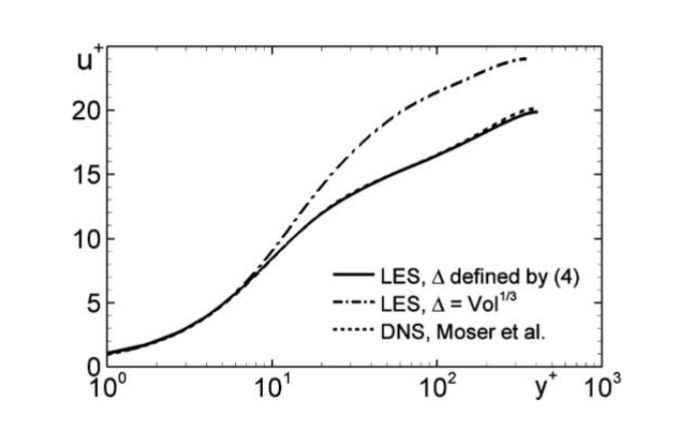
\includegraphics[width = .5\textwidth]{SGSLengthscale.png}
        \caption{Lengthscale experiments for low reynolds wall resolved LES}
    \end{center}
\end{figure}

The second example is WMLES at high reynolds numner $Re_\tau = 18000$ and $Re_\tau = 1100$. 
\begin{figure}[H]
    \begin{center}
        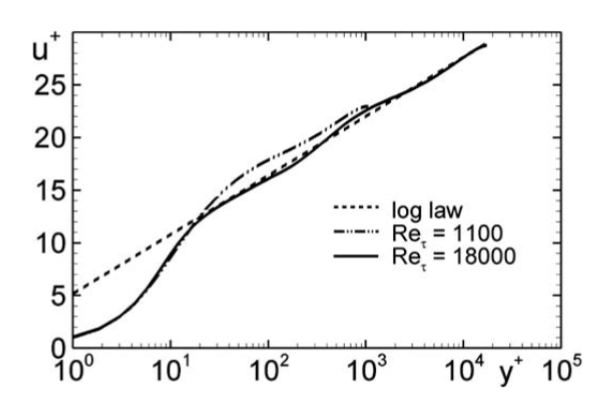
\includegraphics[width = .5\textwidth]{LLM.png}
        \caption{Mean velocity profile of WMLES simulation using proposed lengthscale.}
    \end{center}
\end{figure}
We see that the computed mean velocity profile at the high reynolds number does not have any log layer mismatch and the log law is reproduced fairly well. 


The next few tests explored the WMLES branch of the IDDES framework, i.e. modeling flows with turbulent initial conditions and a sufficiently resolved grid. The following figure demenstrates the profiles o fth blending function $f_d$ and $(1 - f_{dt})$ in a developed channel flow at different $Re_\tau$ with the $k-\omega$ vrsion of IDDES, with initial turbulent content, 
\begin{figure}[H]
    \begin{center}
        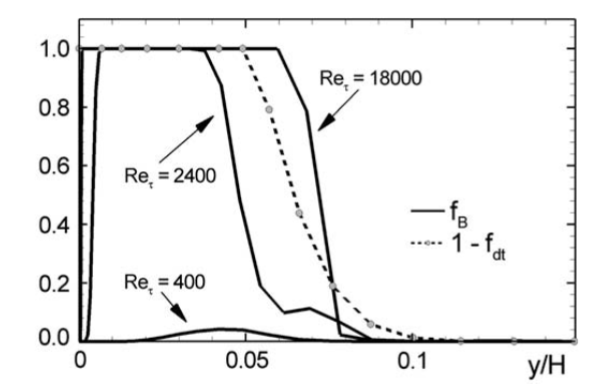
\includegraphics[width = .5\textwidth]{blendingfunction.png}
        \caption{Profiles of lengthscale blending functions in developed channel flow (WMLES case)}
    \end{center}
\end{figure}
We se that at low and moderat $Re_\tau$ $f_B>(1 - f_{dt})$ and therefore the therefore the $f_B$ branch of $f_d$ is active, reducing the hybrid length-scale to the WMLES length-scale. At a high Reynolds number both braches are active with the $(1 - f_{dt})$ branch dominating near the wall and the $f_B$ branch dominating in the outer RANS region. 

% --- Bibliography ---
\newpage
\bibliographystyle{plain}
\bibliography{references}

\end{document} 